%%%%%%%%%%%%%%%%%%%%%%%%%
% Dokumentinformationen %
%%%%%%%%%%%%%%%%%%%%%%%%%
\newcommand{\titleinfo}{Funktionen mehrerer Variablen (Bernhardsgruetter) -
Formelsammlung}
\newcommand{\authorinfo}{F. Braun, Matthias Diethelm und die Schweisser}
\newcommand{\versioninfo}{$Revision: 1021 $ - powered by \LaTeX}

%%%%%%%%%%%%%%%%%%%%%%%%%%%%%%%%%%%%%%%%%%%%%
% Standard projektübergreifender Header für
% - Makros 
% - Farben
% - Mathematische Operatoren 
%
% DORT NUR ERGÄNZEN, NICHTS LÖSCHEN
%%%%%%%%%%%%%%%%%%%%%%%%%%%%%%%%%%%%%%%%%%%%%  
%Schriftgr"osse, Layout, Papierformat, Art des Dokumentes
\documentclass[10pt,a4paper,fleqn,headsepline,footsepline]{scrartcl}
%Einstellungen der Seitenränder
\usepackage[left=0.8cm,right=0.8cm,top=0.5cm,bottom=0.5cm,includeheadfoot]{geometry}
% Sprache, Zeichensatz, packages
\usepackage[UTF8]{inputenc}
\usepackage[ngerman]{babel,varioref}
\usepackage{amssymb,amsmath,graphicx,xcolor,lastpage,wrapfig,verbatim}
\usepackage{tabularx,longtable}
\usepackage{multicol}
\usepackage{rotating}
\usepackage{floatflt}
\usepackage{array}
\usepackage{scrlayer-scrpage}
\usepackage{multirow,multicol}
\usepackage{trfsigns, trsym}
\usepackage{tikz}
\usepackage{circuitikz}
\usepackage{afterpage}

% Zum Bilder einfach in Tabellen einfügen (valign=t)
\usepackage[export]{adjustbox}
%
\setkomafont{pageheadfoot}{\footnotesize}
%
%
\RedeclareSectionCommands[
  beforeskip=.2\baselineskip,
  afterskip=.2\baselineskip
]{section,subsection,subsubsection,paragraph}

\definecolor{pgrey}{rgb}{0.2,0.2,0.2}
\definecolor{black}{rgb}{0,0,0}
\definecolor{red}{rgb}{1,0,0}
\definecolor{white}{rgb}{1,1,1}
\definecolor{grey}{rgb}{0.8,0.8,0.8}
\definecolor{green}{rgb}{0,.8,0.05}
\definecolor{brown}{rgb}{0.603,0,0}

\DeclareMathOperator{\sinc}{sinc}
\DeclareMathOperator{\sgn}{sgn}
\DeclareMathOperator{\Real}{Re}
\DeclareMathOperator{\Imag}{Im}
%\DeclareMathOperator{\e}{e}
\DeclareMathOperator{\cov}{cov}
\DeclareMathOperator{\PolyGrad}{PolyGrad}

\newcommand{\HRule}{\noindent\rule{\linewidth}{1pt}}
%
\newcommand{\myparagraph}[1]{\paragraph{#1}\mbox{}\\\nopagebreak}
\newcommand{\formelbuch}[1]{$\quad{\textcolor{pgrey}{\mbox{\small{S#1}}}}$}
\newcommand{\hartl}[1]{$\quad{\textcolor{pgrey}{\mbox{\small{S#1}}}}$}


\newcommand*{\diff}{\mathop{}\!\mathrm{d}}
\newcommand{\FT}
{
\begin{picture}(1,0.5)
\put(0.2,0.1){\circle{0.14}}\put(0.27,0.1){\line(1,0){0.5}}\put(0.77,0.1){\circle*{0.14}}
\end{picture}
}

\newcommand{\IFT}
{
\begin{picture}(1,0.5)
\put(0.2,0.1){\circle*{0.14}}\put(0.27,0.1){\line(1,0){0.45}}\put(0.77,0.1){\circle{0.14}}
\end{picture}
}


\newcommand{\arraystretchOriginal}{1.3} %%1.5
\renewcommand{\arraystretch}{\arraystretchOriginal}


\newcolumntype{L}[1]{>{\raggedright\let\newline\\\arraybackslash\hspace{0pt}}m{#1}}
\newcolumntype{C}[1]{>{\centering\let\newline\\\arraybackslash\hspace{0pt}}m{#1}}
\newcolumntype{R}[1]{>{\raggedleft\let\newline\\\arraybackslash\hspace{0pt}}m{#1}}


\author{\authorinfo}
\title{\titleinfo}
%
%Kopf- und Fusszeile
%
\lohead*{\titleinfo}
\rohead*{\today}
\lofoot*{\authorinfo}
\cofoot*{
\includegraphics[width=1.6cm]{header/small.png}}
\rofoot*{Seite \thepage { }von \pageref{LastPage}}
%
\pagestyle{scrheadings}




%%%%%%%%%%%%%%%%%%%%
% Generelle Makros %
%%%%%%%%%%%%%%%%%%%%
\newcommand{\prt}[1]{\frac{\partial f}{\partial #1}}
\newcommand{\dprt}[1]{\dfrac{\partial f}{\partial #1}}
\newcommand{\sprt}[1]{\partial_{#1} f}
\newcommand{\fprt}[2]{\frac{\partial #1}{\partial #2}}
\newcommand{\fsprt}[2]{\partial_{#1} #2}

%%%%%%%%%%%%%%%%%%%%%%%%%%%%
% Mathematische Operatoren %
%%%%%%%%%%%%%%%%%%%%%%%%%%%%
\DeclareMathOperator{\gradient}{grad}
\DeclareMathOperator{\rotation}{rot}
\DeclareMathOperator{\divergenz}{div}

% Möglichst keine Ergänzungen hier, sondern in header.tex
\begin{document} 
 

%%%%%%%%%%%%%%%%%%%%%%%%%%%%%%%%%%%%%%%%%%%%%%%%%%%%%%%%%%%%%%%%%%%%%%%%%%%%%%%%%%%%%%%%%%%%%%%
%%%%%%%%%%%%%%%%%%%%%%%%%%%%%%%%%%%%%%%%%%%%%%%%%%%%%%%%%%%%%%%%%%%%%%%%%%%%%%%%%%%%%%%%%%%%%%%

\section{Skalare Funktionen ($\mathbb{R}^n \rightarrow \mathbb{R}$)
\formelbuch{17}}

\subsection{Ableitungen\formelbuch{21}}
\begin{tabular}{|l|l|l|}
\hline
\textbf{partielle Ableitung} & \textbf{Gradient} & \textbf{Richtungsableitung}\\
\hline
\begin{minipage}{5.5cm}
	\vspace{0.2cm}
	$\dprt{x_1}(x_1,\ldots,x_n)= \sprt{x_1}(x_1,\ldots,x_n)$
	\vspace{0.2cm}
\end{minipage}&
\begin{minipage}{6cm}
	$\gradient f(x_1,\ldots,x_n)= \left(\dprt{x_1}, \,\ldots\,,
	\dprt{x_n}\right)$ \end{minipage}&
\begin{minipage}{6.5cm}
	\vspace{0.1cm}
	$D_{\vec{v}}f(x_0,y_0)=\frac{d}{dt}f(x_0+tv_x, y_0+tv_y)|_{t=0}$
	\vspace{0.2cm}\\
	Falls $f$ im Punkt differenzierbar ist gilt: \\
	$D_{\vec{v}}f(x_1,\ldots,x_n)=\gradient f(x_1,\ldots,x_n) \circ \vec{v}$
	\vspace{0.2cm}
\end{minipage}\\
\hline
\begin{minipage}{5.5cm}
	\vspace{0.2cm}
	partielle Ableitung der Funktion $f$ nach dem Parameter $x_1$
	\vspace{0.2cm}
\end{minipage}&
\begin{minipage}{5.5cm}
	Vektor der partiellen Ableitungen von $f$
\end{minipage}&
\begin{minipage}{5.5cm}
	Steigung der Funktion $f$ in Richtung des Vektors $\vec{v}$
\end{minipage}\\
\hline
\end{tabular}

\subsection{Tangentialebene\formelbuch{28}}
$\boxed{g(x,y)=f(x_0,y_0)+\dprt{x}(x_0,y_0)\cdot(x-x_0)+\dprt{y}(x_0,y_0)\cdot(y-y_0)}
\quad \Rightarrow \quad$ Tangentialebene im Punkt $(x_0,y_0,f(x_0,y_0))$\\ \\
$\boxed{\vec{n}(x_0,y_0)=
\begin{pmatrix}
	\sprt{x}(x_0,y_0)\\
	\sprt{y}(x_0,y_0)\\
	-1\\                         
\end{pmatrix}} \quad \Rightarrow \quad$ Normalenvektor der Tangentialebene

\subsection{Niveaulinien und Falllinien\formelbuch{30}}
\textbf{Falllinien, Orthogonaltrajektorien}\\
Falllinien sind Kurven, die in jedem Punkt in Richtung max. Zunahme von f
verlaufen\\
$\Rightarrow \gradient f$ steht tangential zur Falllinie\\\\
$\boxed{y'(x)= \dfrac{\prt{y}}{\prt{x}}} \quad
\Rightarrow \quad$ Steigung der Falllinie $y(x)$\\\\
Durch lösen dieser Differentialgleichung erhält man
die Lösungskurve $y(x)$\\ \\
\textbf{Niveaulinien}\\
$\gradient f \perp $ Niveaulinie\\\\
$\boxed{y'(x)=- \dfrac{\prt{x}}{\prt{y}}}\quad
\Rightarrow \quad$ Steigung der Niveaulinie $y(x)$\\\\
Durch lösen dieser Differentialgleichung erhält man
die Lösungskurve $y(x)$

\subsection{Zusammengesetzte Funktionen\formelbuch{34}}
$\boxed{\gradient(g\circ f)(x)=g'(f(x))\cdot \gradient f(x)}$
\newpage

\subsection{Extremalprobleme\formelbuch{36}}
Extremalstellen einer Funktion $f(x,y)$ bestimmen.\\ \\
\subsection{Extremalprobleme}
\textbf{Zwei Dimensionen}\\
\begin{enumerate}
  \item Randpunkte von $\mathbb{D}_f$
  \item Punkte, in denen der Gradientenvektor $\gradient f$ nicht existiert. 
  \item Punkte, in denen der Gradientenvektor $\gradient f=0$ ist.\\
  Hat die Funktion $f(x;y)$ an der Stelle $(x_0;y_0)$ einen verschwindenden Gradientenvektor $\gradient f = 0$ und gilt für die Diskriminante $\Delta = f_{xx}    (x_0;y_0) \cdot f_{yy}(x_0;y_0) -  (f_{xy}(x_0;y_0))^2$
  \begin{itemize}
    \item $\Delta > 0 $, so besitz $f(x_0;y_0)$ ein lokales Extremum. Im Fall $f_{xx}(x_0;y_0) < 0$ liegt ein lokales Maximum vor, für $f_{xx}(x_0;y_0) >       0$ hingegen ein lokales Minimum.
    \item $\Delta < 0 $, so besitzt $f(x_0;y_0)$ in $(x_0;y_0)$ ein Sattelpunkt.
    \item $\Delta = 0 $, so braucht es weitere Untersuchungen, um die Art der Stelle $(x_0;y_0)$ zu bestimmen können.
    \item Wenn es kein lokales/relatives Minima/Maxima gibt, dann auch kein
    absolutes! 
  \end{itemize}
\end{enumerate}
\textbf{m Dimensionen}\\
Funktion $f(x_1^{(0)};\ldots;x_m^{(0)})$ gegeben.  \\
\begin{itemize}
  \item Schritte 1 - 3 sind gleich wie bei zwei Dimensionen. Kandidaten $(x_1^{(0)};\ldots;x_m^{(0)})$ bekommen.
  \item Bestimmung der Art der Extremalstellen: Hessesche Matrix aufstellen\\
  $H(x_1^{(0)};\ldots;x_m^{(0)}) := \begin{pmatrix}
          f_{x_{1}x_{1}}(x_1^{(0)};\ldots;x_m^{(0)}) & \ldots & f_{x_{1}x_{m}}(x_1^{(0)};\ldots;x_m^{(0)})\\
          \vdots && \vdots\\
          f_{x_{m}x_{1}}(x_1^{(0)};\ldots;x_m^{(0)}) & \ldots & f_{x_{m}x_{m}}(x_1^{(0)};\ldots;x_m^{(0)})
          \end{pmatrix}$\\
  \begin{itemize}
    \item $m$ positive Eigenwerte $\lambda_i > 0$, so besitzt $f$ in $(x_1^{(0)};\ldots;x_m^{(0)})$ ein lokales Minimum,
    \item $m$ negative Eigenwerte $\lambda_i < 0$, so besitzt $f$ in $(x_1^{(0)};\ldots;x_m^{(0)})$ ein lokales Maximum,
    \item positive und negative Eigenwerte, so besitzt $f$ in $(x_1^{(0)};\ldots;x_m^{(0)})$ einen Sattelpunkt.
    \item Wenn $\lambda_i \leqq 0$ oder $\lambda_i \geqq 0$ sind weitere Untersuchungen nötig.
  \end{itemize}
\end{itemize}

\subsubsection{Extremstellen auf Randwerten \formelbuch{38}}
\begin{tabular}{lll}
	\begin{minipage}{3.5cm}
		$\boxed{\gradient f - \lambda \gradient g = 0}$		
	\end{minipage} &
	\begin{minipage}{4.7cm}
		$f: $ zu maximierende Funktion\\
		$g: $ Funktion des Randes	
    \end{minipage} &
	\begin{minipage}{11cm}
		1. Gleichung unter der Bedingung  $g=0$ auflösen\\
		2. Lösungen durch einsetzen in $f$ auf Min o. Max untersuchen
    \end{minipage}
\end{tabular}


\subsection{Extremalprobleme mit Nebenbedingungen}
\textbf{Zwei Dimensionen}\\
Gegeben: $f(x;y)$ unter der Nebenbedingung $n(x;y) = 0$\\
So kommen folgende Punkte von $f$ in Frage:
\begin{enumerate}
  \item Randpunkte von $\mathbb{D}_f$ wenn sie die Nebenbedingungen  $n(x;y) = 0$ erfüllen.
  \item Punkte, in denen der Gradientenvektor $\gradient f $ und / oder $\gradient n$ nicht existiert, und die Nebenbedingung nicht erfüllt ist,
  \item Lösungen des Gleichungsystems\\
  $ \begin{vmatrix}
      f_x(x;y) \cdot n_y(x;y) = f_y(x;y) \cdot n_x(x;y) \\
      n(x;y) = 0
    \end{vmatrix} $
   \item Lösung in $f(x,y)$ einsetzen und untersuchen!
\end{enumerate}

\newpage
\section{Kurven ($\mathbb{R} \rightarrow \mathbb{R}^n$)
\formelbuch{41}}
\subsection{Parametertransformation\formelbuch{42}}
Tangentenrichtung ist unabhängig von der Parametrisierung der Kurve. Die Länge
jedoch nicht. Ist $g$ eine Kurve, beschreibt $f\circ g$ die gleiche Kurve mit
einer anderen Parametrisierung. Der Tangentialvektor ist somit:\\
$$\frac{d(f\circ g)}{dt}(t_0)=\frac{df}{dt}(g(t_0))\frac{dg}{dt}(t_0)=
\frac{df}{dt}(g(t_0))g'(t_0)$$\\
die Länge des Vektors wird also mit dem Faktor $f'(t_0)$ gestreckt oder
gestaucht.

\subsection{Kurvenlänge\formelbuch{42}}
\begin{tabular}{|l||l|l|}
\hline
& \textbf{Formel} & \textbf{Bedingung(en)}\\
\hline
\hline
\textbf{Länge von $a$ nach $b$} &
	\begin{minipage}{5cm}
    	\vspace{0.1cm}
		$L=\int\limits_a^b|{f'(\tau)}|d\tau$ 
		\vspace{0.1cm}
    \end{minipage}&
rektifizierbar $\quad\Rightarrow\quad f'(t)$ integrierbar\\
\hline
\textbf{Länge in Abhängigkeit der Zeit} &
	\begin{minipage}{5cm}
    	\vspace{0.1cm}
		$s(t)=\int\limits_a^t|{f'(\tau)}|d\tau$ 
		\vspace{0.1cm}
    \end{minipage}&
\begin{minipage}{7cm}
	rektifizierbar $\quad\Rightarrow\quad f'(t)$ integrierbar\\
	regulär $\qquad\quad\;\;\Rightarrow\quad f'(t)\neq 0$
\end{minipage}\\
\hline
\end{tabular}\vspace{0.5cm}\\

\textbf{Kurve in Kurvenlängenparameter transformieren}
\begin{enumerate}
  \item Prüfen ob $f'(t)\neq 0$ \& integrierbar ist, falls nicht kann die Kurve
  nicht transformiert werden.
  \item $s(t)$ berechnen.
  \item Umkehrfunktion $s(t)^{-1}$ berechnen.
  \item $t(s)$ in $f$ einsetzen $\Rightarrow f(t(s))= f\circ s(t)^{-1}$
\end{enumerate}
\vspace{0.5cm}
\textbf{Eigenschaften für Kurvenlängenparameter}\\
Eine Kurve besitzt Kurvenlängenparameter wenn folgendes gilt:\\
$$\left|\frac{df}{dt}(t)\right|=1$$

\subsection{Krümmung \& Krümmungskreisradius\formelbuch{45}}
\begin{tabular}{|l|l|l|}
	\hline
	& mit Kurvenlägenparameter & ohne Kurvenlängenparameter\\
	\hline
	Krümmung &
	$\kappa(s)=|f''(s)|$ &
	\begin{minipage}{5cm}
    	\vspace{0.1cm}
		$\kappa(t)=\dfrac{|f'(t) \times f''(t)|}{|f'(t)|^3}$\\ 
		\vspace{0.1cm}
    \end{minipage}\\	
	\hline
	Krümmungskreisradius &
	$r(s)=\dfrac{1}{\kappa(s)}=\dfrac{1}{|f''(s)|}$ &
	\begin{minipage}{5cm}
    	\vspace{0.1cm}
		$r(t)=\dfrac{1}{\kappa(t)}=\dfrac{|f'(t)|^3}{|f'(t) \times
		f''(t)|}$    
		\vspace{0.1cm}
    \end{minipage}\\
	\hline
\end{tabular}
\newpage

\newpage
\section{Abbildungen ($\mathbb{R}^n \rightarrow \mathbb{R}^m$)
\formelbuch{55}}
\subsection{Ableitungen\formelbuch{55}}
$Df(x) = \begin{pmatrix}
    	\fprt{f_1}{x_1}(x) & \ldots & \fprt{f_1}{x_n}(x)\\
    	\vdots && \vdots\\
    	\fprt{f_m}{x_1}(x) & \ldots & \fprt{f_m}{x_n}(x)
	\end{pmatrix}=\dfrac{\partial(f_1,\ldots,f_m)}{\partial(x_1,\ldots,x_n)}
	\quad \Rightarrow \quad$ Jacobi-Matrix (Ableitung in alle Koordinatenrichungen)
\subsection{Kettenregel\formelbuch{56}}
\begin{minipage}{3cm}
	$f: \mathbb{R}^n \rightarrow \mathbb{R}^m$\\
	$g: \mathbb{R}^m \rightarrow \mathbb{R}^r$
\end{minipage}
\begin{minipage}{7cm}
	$\boxed{h=D(g\circ f)(x)=Dg(f(x_0))\cdot Df(x_0)}$
\end{minipage}
\begin{minipage}{4cm}
	$h: \mathbb{R}^n \rightarrow \mathbb{R}^r$
\end{minipage}

\subsection{Volumenänderung\formelbuch{58}}
$\Delta V = \begin{vmatrix}
    	\fprt{f_1}{x_1}(x) & \ldots & \fprt{f_1}{x_n}(x)\\
    	\vdots && \vdots\\
    	\fprt{f_m}{x_1}(x) & \ldots & \fprt{f_m}{x_n}(x)
		\end{vmatrix}=\left|\dfrac{\partial(f_1,\ldots,f_m)}
		{\partial(x_1,\ldots,x_n)}\right|= det Df$

\subsection{Newtonverfahren\formelbuch{60}}
Mit dem Newtonverfahren können rekursiv Nullstellen approximiert werden.\\\\
$\boxed{\vec{x}_{neu}=\vec{x}_{alt}-(Df(\vec{x}_{alt}))^{-1}\cdot
(f(\vec{x}_{alt})-\vec{y}_{Ziel})}\qquad$ allgemein\\
$\boxed{x_{neu}=x_{alt}-(f'(x_{alt}))^{-1}\cdot
(f(x_{alt})-y_{Ziel})}\qquad$ (1- Dimensional) wird
rekursiv ausgeführt, bis nötige Genauigkeit da ist.

\section{Mehrfache Integrale \formelbuch{67}}
\subsection{Oberflächenberechnung\formelbuch{73}}
\begin{tabular}{|p{5.5 cm}|p{10cm}|}
	\hline
	\begin{minipage}{5.5cm}
    	\vspace{0.1cm}
    	Oberflächenintegral\\
    	$f:G\rightarrow \mathbb{R}$
    	\vspace{0.1cm} 
    \end{minipage}&
	\begin{minipage}{10cm}
    	\vspace{0.1cm}
		$F = \iint\limits_G \sqrt{(\sprt{x})^2+(\sprt{y})^2+1}\cdot d\mu$
    	\vspace{0.1cm}
    \end{minipage}\\
	\hline
	\begin{minipage}{5.5cm}
    	\vspace{0.1cm}
    	Oberflächenintegral\\
    	$f:G\rightarrow \mathbb{R}^3$
    	\vspace{0.1cm} 
    \end{minipage}&
	\begin{minipage}{10cm}
    	\vspace{0.1cm}
		$F=\iint\limits_G\left|
		\begin{pmatrix}
	    	\fsprt{x}{f_1}\\
	    	\fsprt{x}{f_2}\\
	    	\fsprt{x}{f_3}\\              
	    \end{pmatrix}
		\times
		\begin{pmatrix}
	      	\fsprt{y}{f_1}\\
	    	\fsprt{y}{f_2}\\
	    	\fsprt{y}{f_3}\\   	
	    \end{pmatrix}\right|d\mu=
		\iint\limits_G |D_1f\times D_2f|\cdot d\mu$	
    	\vspace{0.1cm}
    \end{minipage}\\
	\hline
	\begin{minipage}{5.5cm}
  		Mantelfläche eines Rotationskörpers in Zylinderkoordinaten    
    \end{minipage}&
	\begin{minipage}{10cm}
    	\vspace{0.1cm}
		$M = 2\pi\int\limits_0^h\varrho(z)\sqrt{1+\varrho'(z)^2}\cdot dz$
    	\vspace{0.1cm}
    \end{minipage}\\
	\hline
	Polarkoordinaten &
	\begin{minipage}{10cm}
    	\vspace{0.1cm}
		$F=\iint\limits_G f(r,\varphi)\cdot \textcolor{blue}{r} \cdot dr d\varphi $
    	\vspace{0.1cm}
    \end{minipage}\\
	\hline
\end{tabular}

\subsection{Volumenberechnung\formelbuch{67 \& 76}}
\begin{tabular}{|p{6 cm}|p{10cm}|}
	\hline
	Allgemein mit Variablentransformation &
	\begin{minipage}{10cm}
    	\vspace{0.1cm}
		$V=\iiint\limits_G f(x,y,z)\cdot dxdydz=\iiint\limits_G f(g(u,v,w))\cdot
		\textcolor{blue}{detDf}\cdot dudvdw$
    	\vspace{0.1cm}
    \end{minipage}\\
	\hline
	Zylinderkoordinaten &
	\begin{minipage}{10cm}
    	\vspace{0.1cm}
		$V=\iiint\limits_G f(r,\varphi,z)\cdot \textcolor{blue}{r} \cdot
		dr d\varphi dz$
    	\vspace{0.1cm}
    \end{minipage}\\
	\hline
	Kugelkoordinaten &
	\begin{minipage}{10cm}
    	\vspace{0.1cm}
		$V=\iiint\limits_G f(r,\varphi,\vartheta)\cdot \textcolor{blue}{r^2
		\cos\vartheta} \cdot dr d\varphi d\vartheta$
    	\vspace{0.1cm}
    \end{minipage}\\
	\hline	
\end{tabular}

\subsection{Schwerpunkt\formelbuch{78} und Trägheitsmoment\formelbuch{79} }
$\boxed{\vec{S}=\begin{pmatrix}
	x_s\\
	y_s\\
	z_s                                            
\end{pmatrix}=\frac{1}{M}\iiint\limits_G \varrho(x,y,z) \cdot
\begin{pmatrix}
	x\\
	y\\
	z                                            
\end{pmatrix}\cdot dxdydz \quad M=\iiint\limits_G \varrho(x,y,z) \cdot
dxdydz}$\\

$x_s=\frac{1}{M} \int\limits_F x \cdot \varrho(x,y,z)\cdot dV\\
y_s=\frac{1}{M} \int\limits_F y \cdot \varrho(x,y,z)\cdot dV\\$
mit $\varrho$ konstant und Objekt nur Platte ($z$ entfaellt):\\
$
x_s=\frac{1}{F} \int\limits_F x\cdot dF = \frac{1}{F} \int\limits_a^b
x(y_0(x)-y_u(x))\cdot dx\\
y_s=\frac{1}{F} \int\limits_F y\cdot dF = \frac{1}{2F} \int\limits_a^b
(y_0^2(x)-y_u^2(x))\cdot dx$\\

$\boxed{I=\iiint\limits_G \varrho(x,y,z)\cdot
\underbrace{(x^2+y^2)}_{k}\cdot
dxdydz}\quad k$ entspricht dem Abstand zur Rotationsachse hier die $Z$-Achse





\newpage
\section{Vektorfelder\formelbuch{83}}
Ein Vektorfeld ist eine Abbildung $\vec{v}:\mathbb{R}^n\rightarrow
\mathbb{R}^n$, welche jedem Punkt des Raumes einen Vektor anheftet.
\subsection{Wegintegral\formelbuch{83}}
Ist $\vec{F}$ ein Vektorfeld und $C:\vec{c}=\vec{c}(t),a\leq t \leq b$ eine
Kurve, dann wird das Wegintegral wie folgt berechnet:\\\\
$\boxed{\int\limits_C\vec{F}\cdot d\vec{s}=
\int\limits_a^b\vec{F}(\vec{c}(t))\cdot \dot{\vec{c}}(t)\cdot dt}$\\\\
Tipp: Wenn c bspw. eine gerade Linie vom Punkt (-1;0) bis (1;0) ist, dann ist:\\
$\vec{c}(t)=
  \begin{pmatrix}
      x(t)\\
      y(t)\\
  \end{pmatrix}
  =
    \begin{pmatrix}
      t\\
      0\\
  \end{pmatrix}$
  mit $-1\leq t \leq 1$

\textbf{Eigenschaften des Wegintegrals}
\begin{itemize}
  \item Ist $C$ eine geschlossene Kurve, also $\vec{c}(a)=\vec{c}(b)$, spricht
  man von einem \textbf{Umlaufintegral} und verwendet folgende Definition:
  $\oint\limits_C \vec{F}\cdot d\vec{s}$
  \item Ist $C=C_1+C_2$ gilt folgendes:$\quad\int\limits_C \vec{F}\cdot
  d\vec{s}=\int\limits_{C_1} \vec{F}\cdot d\vec{s}+\int\limits_{C_2}
  \vec{F}\cdot d\vec{s}$
  \item Wird $C$ in Gegenrichtung durchlaufen gilt folgendes:
  $\quad\int\limits_C \vec{F}\cdot
  d\vec{s}=-\int\limits_{-C} \vec{F}\cdot d\vec{s}$
\end{itemize}

\subsection{Konservative Felder / Potentialfelder\formelbuch{84}}
Ein Vektorfeld $\vec{v}$ heisst \textit{konservativ}, wenn das Wegintegral
unabhängig vom gewählten Weg ist.\\\\
$\Rightarrow\qquad \boxed{\oint_C \vec{v}\cdot d\vec{s}=0}\qquad\boxed{
\int\limits_{Weg_1\, A\rightarrow B} \vec{v}\cdot d\vec{s}=\int\limits_{Weg_2\,
A\leadsto B} \vec{v}\cdot d\vec{s}=\int\limits_A^B \vec{v}\cdot
d\vec{s}}\qquad\boxed{\rotation (\vec{v})=0}$\\\\\\	
\textbf{Es gelten folgende zwei Sätze:}
\begin{itemize}
  \item Ist $\vec{v}=\gradient f$, dann ist $\vec{v}$
  \textit{konservativ} und es gilt: $\quad\int\limits_A^B \vec{v}\cdot d\vec{s}=f(B)-f(A)$
  \item Ist $\vec{v}$ \textit{konservativ}, dann gibt es eine Funktion $f$ so,
  dass $\vec{v}=\gradient f$.
\end{itemize}

\subsection{Rotation\formelbuch{86 \& 92}}
Interpretiert man dieses Feld als Strömungsfeld, so gibt die Rotation für jeden
Ort an, wie schnell und um welche Achse ein mitschwimmender Körper rotieren
würde. Ein Vektorfeld, dessen Rotation überall null ist, nennt man
\textit{wirbelfrei}.\\\\
\begin{minipage}{8cm}
	\textbf{2-Dimensional}\\\\
	$\boxed{\rotation(u,v)=\fprt{v}{x}-\fprt{u}{y}}$
\end{minipage}
\begin{minipage}{8cm}
	\textbf{3-Dimensional}\\\\
	$\boxed{\rotation(u,v,w)=\bigtriangledown\times
	\vec{v}=
	\begin{pmatrix}
    	\partial_x\\
    	\partial_y\\
    	\partial_z
    \end{pmatrix}\times
	\begin{pmatrix}
    	v_x\\
    	v_y\\
    	v_z
    \end{pmatrix}=
	\begin{pmatrix}
    	\fsprt{y}{w}-\fsprt{z}{v}\\
    	\fsprt{z}{u}-\fsprt{x}{w}\\
    	\fsprt{x}{v}-\fsprt{y}{u}
    \end{pmatrix}}$
\end{minipage} \\

\subsection{Divergenz\formelbuch{96}}
Interpretiert man dieses Feld als Strömungsfeld, so gibt die Divergenz für jede
Stelle die Tendenz an, ob ein Teilchen in der Nähe zu diesem Punkt hin- bzw.
von diesem Punkt wegfließt. Es sagt damit aus, ob und wo das Vektorfeld Quellen
(Divergenz größer als Null) oder Senken (Divergenz kleiner als Null) hat. Ist
die Divergenz überall gleich Null, so bezeichnet man das Feld als
\textit{quellenfrei}.\\\\
$\boxed{\divergenz \vec{v}=\bigtriangledown\circ \vec{v}=
	\begin{pmatrix}
    	\partial_{x_1}\\
    	\vdots\\
    	\partial_{x_n}
    \end{pmatrix}\cdot
	\begin{pmatrix}
    	v_{x_1}\\
    	\vdots\\
    	v_{x_n}
    \end{pmatrix}=
\sum\limits_{i=1}^n \fprt{v_i}{x_i}}$

\subsection{Fluss\formelbuch{93}}
Der Fluss des Vektorfeldes $\vec{v}$ durch das Flächenstück G mit
Parametrisierung $f:U\rightarrow\mathbb{R}^3$ ist:\\\\
$\boxed{\iint\limits_G\vec{v}\cdot d\vec{n}=\iint\limits_U \vec{v}\cdot
(\sprt{u}\times\sprt{v}) dudv}$

\subsection{Integralsätze}
	\begin{tabular}{|p{0.4cm}||p{4cm}|p{5.7cm}|p{7cm}|}
	\hline
	& \textbf{Satz} & \textbf{Formel} & \textbf{Beschreibung}\\
	\hline
	\hline
	\begin{sideways}2-D \qquad \end{sideways} &
  	Die Greensche Formel \formelbuch{88} &
	\begin{minipage}{6.7cm}
	    \vspace{0.1cm}
		$\int\limits_{\partial G}\vec{v}\cdot d\vec{s}=\iint\limits_G \rotation
		\vec{v}\cdot d\mu$	 		    
	    \vspace{0.1cm}   
    \end{minipage}&
	\begin{minipage}{7cm}
	    \vspace{0.1cm}
		Die Greensche Formel beschreibt den Zusammenhang zwischen einem
		\textbf{Wegintegral} und einem \textbf{Oberflächenintegral}.
	    \vspace{0.1cm}   
    \end{minipage}\\
	\hline
	\begin{sideways}3-D \qquad \end{sideways} &
	Der Satz von Stokes \formelbuch{94} &
	\begin{minipage}{6.7cm}
    	\vspace{0.1cm}
		$\int\limits_{\partial G}\vec{v}\cdot d\vec{s}=\iint\limits_G \rotation
		\vec{v}\cdot d\vec{n}$		 
		\vspace{0.1cm} 
    \end{minipage}&
	\begin{minipage}{7cm}
    	\vspace{0.1cm}
		Der Satz von Stokes definiert einen Zusammenhang zwischen einem
		\textbf{Wegintegral} und einem \textbf{Flussintegral}.	    
	    \vspace{0.1cm}   
    \end{minipage}\\
	\hline
	\begin{sideways}3-D \qquad \end{sideways} &
	Der Satz von Gauss \formelbuch{96} &
	\begin{minipage}{6.7cm}
	    \vspace{0.1cm}
		$\iint\limits_{\partial V}\vec{v}\cdot d\vec{n}=\iiint\limits_V \divergenz
		\vec{v}\cdot dV$			    
	    \vspace{0.1cm}   
    \end{minipage}&
	\begin{minipage}{7cm}
    	\vspace{0.1cm}
		Der Satz von Gauss definiert einen Zusammenhang zwischen einem
		\textbf{Flussintegral} und einem \textbf{Volumenintegral}.	    
	    \vspace{0.1cm}    
    \end{minipage}\\
	\hline	
\end{tabular}

\section{Diverses}
\subsection{Koordinatensysteme}
\begin{tabular}{|p{2.5cm}||p{3cm}|p{4.2cm}|p{7.5cm}|}
	\hline
	$f(x,y,(z))\quad\rightarrow$ &
	\begin{minipage}{2.4cm}
    	\vspace{0.1cm}
		$f(r,\varphi)\quad$\textbf{Polar} 
    	\vspace{0.1cm}    	
    \end{minipage}& 
	$f(r,\varphi,z)\quad$ \textbf{Zylinder} &
	$f(r,\varphi,\vartheta)\quad$\textbf{Kugel}\\
	\hline
	\hline
	Bilder &
	\begin{minipage}{3cm}
    	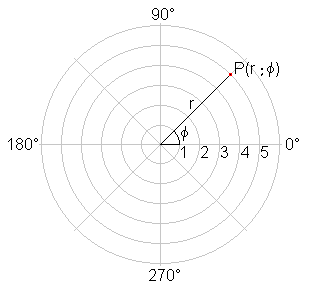
\includegraphics[width=3cm]{../FuVar/images/Ebene_polarkoordinaten.png}
    \end{minipage}&
	\begin{minipage}{3cm}
    	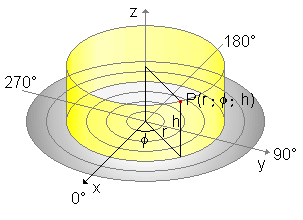
\includegraphics[width=4.2cm]{../FuVar/images/Zylinderkoordinaten.png}
    \end{minipage}&
	\begin{minipage}{3cm}
    	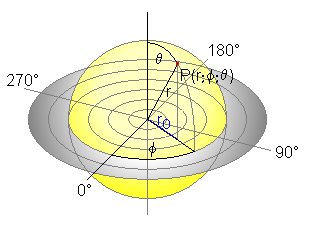
\includegraphics[width=5cm]{../FuVar/images/Kugelkoordinaten.png}
    \end{minipage}\\
	\hline
	Umrechnungs- formeln &
	\begin{minipage}{3cm}
    \vspace{0.1cm}
		$x=r\cos\varphi$\\
		$y=r\sin\varphi$    
    \vspace{0.1cm}
    \end{minipage}&	
	\begin{minipage}{4.2cm}
    \vspace{0.1cm}
    	$x=r\cos\varphi$\\
    	$y=r\sin\varphi$\\
    	$z=z$
    \vspace{0.1cm}
    \end{minipage}&	
	\begin{minipage}{7.5cm}
    \vspace{0.1cm}
    	$x=r\sin\vartheta\cos\varphi$\\
    	$y=r\sin\vartheta\sin\varphi$\\
    	$z=r\sin\vartheta$
    \vspace{0.1cm}
    \end{minipage}\\
	\hline
	Jacobi-Matrix $Df$ &
	\begin{minipage}{3cm}
    \vspace{0.1cm}
		$\begin{pmatrix}
         	\cos\varphi & -r\sin\varphi\\
         	\sin\varphi & r\cos\varphi
         \end{pmatrix}$
    \vspace{0.1cm}
    \end{minipage}&	
	\begin{minipage}{4.2cm}
    \vspace{0.1cm}
		$\begin{pmatrix}
         	\cos\varphi & -r\sin\varphi & 0\\
         	\sin\varphi & r\cos\varphi & 0\\
         	0 & 0 & 1
         \end{pmatrix}$
    \vspace{0.1cm}
    \end{minipage}&	
	\begin{minipage}{7.5cm}
    \vspace{0.1cm}
		$\begin{pmatrix}
         	\sin\vartheta\cos\varphi & -r\sin\vartheta\sin\varphi &
         	r\cos\vartheta\cos\varphi\\
         	\sin\vartheta\sin\varphi & r\sin\vartheta\cos\varphi &
         	r\cos\vartheta\sin\varphi\\
         	\cos\vartheta & 0 & -r\sin\vartheta
         \end{pmatrix}$
    \vspace{0.1cm}
    \end{minipage}\\
	\hline
	\begin{minipage}{2.5cm}
    	\vspace{0.1cm}
  		$detDf$   
  		\vspace{0.1cm}
    \end{minipage}&
		$r$ &
		$r$ &
		$r^2\cos\vartheta$\\
	\hline	
\end{tabular}

\subsection{Rechenregeln für div, rot, grad, $\Delta$}
\begin{minipage}{9cm}
Sei $D \in \mathbb{R}^3, f \in C^2(D,\mathbb{R}), \vec{v} \in C^2(D,\mathbb{R}^3)$. Dann gilt:
\begin{itemize}
	\item $\rotation(\gradient f) = 0 \qquad $ ``Gradientenfeld ist wirbelfrei''
	\item $\divergenz(\rotation \vec{v}) = 0 \qquad $ ``Feld der Rotation ist quellfrei''
	\item $\divergenz(\gradient f) = \Delta f$
	\item $\divergenz(f\vec{v}) = (\gradient f) \cdot \vec{v} + f \divergenz \vec{v}$
	\item $\rotation(f\vec{v}) = (\gradient f) \times \vec{v} + f \rotation \vec{v}$
	\item $\rotation(\rotation \vec{v}) = \gradient(\divergenz \vec{v}) - \Delta \vec{v}$
\end{itemize}
(Laplace–Operator kompomentenweise anwenden!) .
\end{minipage}
\hspace{1cm}
\begin{minipage}[b]{6cm}
\textbf{Laplace-Operator($\Delta$):}\\
$\Delta=\vec\nabla^2= \sum_{k=1}^n {\partial^2\over \partial x_k^2}$\\\\
\textbf{ Nabla-Operator($\nabla$):}\\
$\vec\nabla = \left (\frac\partial{\partial x_1},\ldots, \frac\partial{\partial
x_n}\right) $
\end{minipage}

%%%%%%%%%%%%%%%%%%%%%%%%%%%%%%%%%%%%%%%%%%%%%%%%%%%
% Idiotenseite
%%%%%%%%%%%%%%%%%%%%%%%%%%%%%%%%%%%%%%%%%%%%%%%%%%%
\newpage
\section{Idiotenseite}
\input{idiotenseite/trigo/subsections/Winkelargumente}
\input{idiotenseite/trigo/subsections/Periodizitaet}
\input{idiotenseite/trigo/subsections/Quadrantenbeziehungen}
\begin{multicols}{2}
  \input{idiotenseite/trigo/subsections/Additionstheoreme}
  \columnbreak
  
  \input{idiotenseite/trigo/subsections/DoppelHalbwinkel}
\end{multicols}
\begin{multicols}{2}
  \input{idiotenseite/trigo/subsections/Produkte}
  \columnbreak
  
  \input{idiotenseite/trigo/subsections/SummeDifferenzen}
\end{multicols}
\input{idiotenseite/diverses/subsections/unbestimmteIntegrale}



%\newpage
%\section{Übungsverzeichnis}
\renewcommand{\arraystretch}{1.05}
\begin{tabular}{|l|l|l|l|}
\hline
\textbf{Thema} & \textbf{Übung} & \textbf{Probeprüfung} & \textbf{Modulprüfung 07} \\ \hline
Achsabschnitte der Tangentialebene & 2.2 &  &  \\ \hline
Approximation mit Tangentialebene & 2.3 &  &  \\ \hline
Bogenlängenparameter &  & 4 &  \\ \hline
Definitionsbereich & 1.2 &  &  \\ \hline
Differenzialgleichung &  &  & 3 \\ \hline
Differenzierbarkeit &  & 2 &  \\ \hline
Divergenz & 13.3 / 13.4 & 8 &  \\ \hline
Elektromagnetisches Feld & 13.4 &  &  \\ \hline
Extremalprobleme & 4.3 &  &  \\ \hline
Extremalstellen auf Randwerten & 5.1 / 5.2 &  &  \\ \hline
Falllinien & 4.2 & 9 &  \\ \hline
Feldstärke in Abhängigkeit vom Radius & 13.2 &  &  \\ \hline
Flächenänderung & 7.3 &  &  \\ \hline
Flächenberechnung mit der Greenschen Formel & 11.4 &  &  \\ \hline
Flugzeug am exponentiellen Berg & 3.5 &  &  \\ \hline
Fluss & 12.2 / 12.3 / 13.1 &  &  \\ \hline
Gauss (Satz) & 13.1 &  &  \\ \hline
Gebiete & 8.1 & 8 &  \\ \hline
Gradient & 3.1 &  &  \\ \hline
Greensche Formel & 11.2 / 11.3 &  & 8 \\ \hline
Grenzwerte eines Gradienten & 3.6 &  &  \\ \hline
Implizite Differentiation & 4.1 &  &  \\ \hline
Insektenmännchen & 3.4 &  &  \\ \hline
Jacobimatrix & 7.2 / 7.3 / 7.4 &  &  \\ \hline
Krümmung / Krümmungsradius & 5.3 & 4 &  \\ \hline
Krümmungmittelpunkt & 5.4 &  &  \\ \hline
Maximieren einer Funktion & 5.1 / 5.2 & 5 & 5 \\ \hline
Maximum & 4.3 & 1 &  \\ \hline
Mehrfachintegrale & 8.2 / 8.3 / 8.4 & 3 & 1 / 4 / 7 \\ \hline
Minimum & 4.3 & 1 &  \\ \hline
Newtonverfahren & 7.1 / 7.2 / 7.5 &  &  \\ \hline
Niveaulinien & 3.3 &  &  \\ \hline
Oberflächenberechnung & 9.3 / 10.3 &  &  \\ \hline
Parameterdarstellung &  & 3 & 1 \\ \hline
Partielle Ableitung & 2.1 &  &  \\ \hline
Pfadintegral, Wegintegral & 6 / 11.2 & 7 & 8 \\ \hline
Potentialfeld & 6 / 11.1 &  & 6 \\ \hline
Richtungsableitung &  & 2 &  \\ \hline
Rotation & 11.1 &  &  \\ \hline
Rotationskörper & 9.1 / 9.2 &  &  \\ \hline
Sattelpunkt & 4.3 & 1 &  \\ \hline
Schnittkurve von zwei Funktionen & 2.4 &  &  \\ \hline
Schwerpunkt berechnen & 10.1 / 10.2 / 10.3 / 10.4 &  &  \\ \hline
Steigung impliziter Funktionen & 4.1 &  &  \\ \hline
Stokes (Satz) & 12.1 &  & 6 \\ \hline
Tangentialebene & 2.2 / 2.3 &  &  \\ \hline
Trägheitsmoment & 10.2 & 6 &  \\ \hline
Volumenänderung & 7.4 &  &  \\ \hline
Volumenberechnung & 8.2 / 8.3 / 8.4 / 9.1 / 9.2 & 3 & 1 / 4 / 7 \\ \hline
Wertebereich & 1.2 &  &  \\ \hline
Winkel zwischen zwei Funktionen & 2.4 &  &  \\ \hline
\end{tabular}

\renewcommand{\arraystretch}{1}

\end{document}
